\section{Metodi di decomposizione strutturale e Isole di tracciability per problemi NP-Hard}

Stiamo partendo da questo grafico per quanto riguarda il \textbf{Kakutani's
    fixed point theorem}:

\begin{figure}[H]
    \centering
    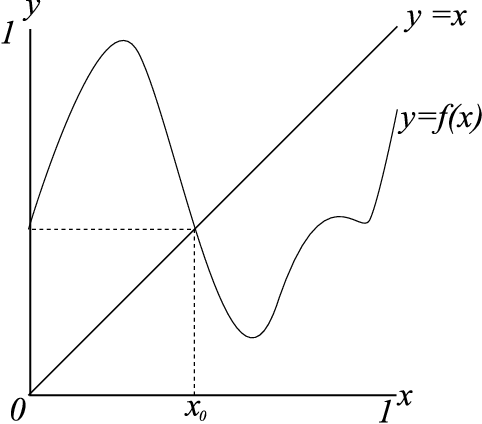
\includegraphics[width=0.7\linewidth]{chapters/images/13-Figure1.1-1.png}
    \caption{}
    \label{fig:1}
\end{figure}

dove sull'asse delle $x$ abbiamo la \textbf{probabilità di fare un'azione}, e
sull'asse delle $y$ la nuova probabilità di eseguire quell'azione.

\[
    x \rightarrow y
\]

ma x e y sono la stessa cosa. E' una funzione che va in se stessa.

Il momento in cui si interseca la bisezione del quadrante, sei sicuro che
\textbf{quel punto esiste} e che quel punto è un \textbf{equilibrio di Nash}.

Non ho la minima idea di cosa stia succedendo qui, ma vediamo cosa ha da dire
chat.

\textit{Risposta di Copilot Chat:}

Nella teoria dei giochi, il teorema del punto fisso di Kakutani è usato per
dimostrare l'esistenza dell'equilibrio di Nash. Un equilibrio di Nash è una
situazione in cui nessun giocatore può migliorare il proprio risultato
cambiando unilateralmente la propria strategia, dato che le strategie degli
altri giocatori rimangono invariate.

La connessione tra il teorema del punto fisso di Kakutani e l'equilibrio di
Nash è la seguente: si può pensare a ogni strategia come a un punto in uno
spazio, e a ogni risposta ottimale a una strategia come a un altro punto in
quello spazio. L'equilibrio di Nash corrisponde a un punto fisso in questo
spazio: un punto che è mappato su se stesso dalla funzione che assegna a ogni
strategia la sua risposta ottimale.

In altre parole, l'equilibrio di Nash è una situazione in cui la "migliore
risposta" di ogni giocatore alla strategia degli altri è semplicemente la
strategia che sta già giocando. Questo è esattamente il tipo di situazione che
il teorema del punto fisso di Kakutani è progettato per gestire, quindi può
essere usato per dimostrare che un tale equilibrio deve esistere.

Nei giochi \textbf{puri}, \textit{trovare} un equilibro di nash è
\textbf{NP-Complete}. E nel caso dei giochi \textbf{misti}, in quale
complessità siamo?

Nei giochi misti sappiamo subito che la risposta è \textbf{si!}, ma dalla
\textit{proof} si vede che non è facile trovare il valore di $f$. In
letteratura, si è visto che in questi casi si può ottenere un equilibro di nash
con valore \textit{irrazionale}, come $\frac{1}{\sqrt{2}}$.

\begin{equation}
    \begin{aligned}
        a_i , b_i, c_i                                     \\
        \text{utility} = f(\sum a_i \times b_i \times c_i) \\
        \text{Si può ottenere } \sqrt{3}
    \end{aligned}
\end{equation}

E alla lavagna ha scritto, rispettivamente come per i giochi puri
\textbf{np-complete}, per i giochi misti ha scritto \textbf{computazione}.

\subsection{PPAD} ( Polynomial Parity Argument on Directed Graphs )

C'è un grafo particolare per questa complessita, che è il seguente:

%6 nodi, 4 hanno un ciclo, il terzo va ad un altro nodo, questo altro nodo va in un altro e uno va fuori, l'altro nodo va al 4o

A quanto pare navigare questo grafo era importante e rappresentava qualcosa, ma
purtroppo non ho capito perché è letteralmente andato come un razzo e non c'è
assolutamenteniente su internet di quello che diceva Greco.

\subsection{Tree Decomposition}

Partiamo a parlare di complessità esponenziale. L'esempio principale è quello
del \textbf{domino}. Il domino è un gioco che si gioca con delle tessere, che
hanno due numeri da 0 a 6, e si devono mettere in fila in modo che i numeri
combacino. Il gioco è finito quando non si possono più mettere tessere in fila.

In generale, dato un insieme di tessere, siamo in grado di mettere in uno
spazio limitato? Si, è NP-Hard: si guessa e si controlla. Ma se vogliamo fare
la stessa cosa per uno spazio senza limiti, come facciamo? Il problema è
esponenziale.

\begin{esempio}(3 colorabilità)
\end{esempio}

\begin{itemize}
    \item Input: Un grafo $G$
    \item Domanda: Il grafo $G$ è 3-colorabile?
\end{itemize}

%disegna un grafo 3 colorabile
\begin{figure}[H]
    \begin{center}
        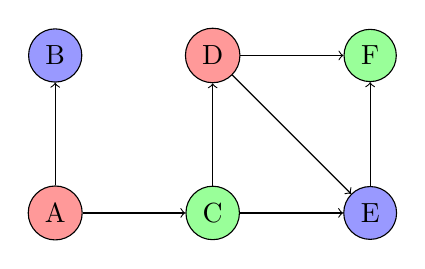
\begin{tikzpicture}
            \node[shape=circle,draw=black,fill=red!40] (A) at (0,0) {A};
            \node[shape=circle,draw=black,fill=blue!40] (B) at (0,2) {B};
            \node[shape=circle,draw=black,fill=green!40] (C) at (2,0) {C};
            \node[shape=circle,draw=black,fill=red!40] (D) at (2,2) {D};
            \node[shape=circle,draw=black,fill=blue!40] (E) at (4,0) {E};
            \node[shape=circle,draw=black,fill=green!40] (F) at (4,2) {F};
            \path [->] (A) edge node[left] {} (B);
            \path [->] (A) edge node[left] {} (C);
            \path [->] (C) edge node[left] {} (D);
            \path [->] (C) edge node[left] {} (E);
            \path [->] (D) edge node[left] {} (E);
            \path [->] (D) edge node[left] {} (F);
            \path [->] (E) edge node[left] {} (F);
        \end{tikzpicture}
    \end{center}
\end{figure}

Parola chiave: \textbf{i cicli}. A quanto pare i cicli sono il \textbf{male} in
informatica.

Il problema della 3 colorabiltà è \textbf{NP-Hard}, ma se abbiamo controllo sui
grafi e sui cicli, il problema cambia. Dobbiamo creare una \textbf{metrica} che
ci permetta di gestire questa cosa: \textbf{gradi di ciclicità di un grafo} (In
inglese, \textit{degree of cyclicity})

\begin{domanda}(Come definiamo un grafo senza cicli)
    Un albero è una struttura dati che può essere definita un grafo senza cicli.
\end{domanda}

Banalmente, \textit{se vediamo il grafo come un albero}, il problema della 3
colorabilità diventa \textbf{triviale}. \textbf{Non c'è bisogno di modificare
    le scelte precedenti}, perché per ogni nodo sai quale colore scegliere per i
figli; non c'è più bisogno di un algoritmo di backtracking.

%disegna il grafo di prima come un albero 

\begin{figure}[H]
    \begin{center}
        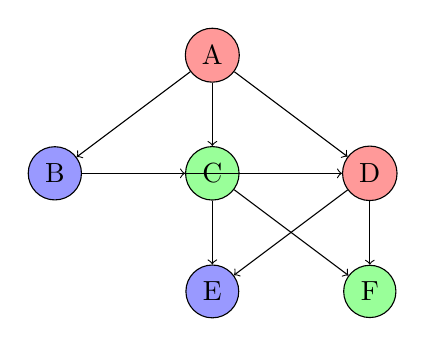
\begin{tikzpicture}
            \node[circle,draw=black,fill=red!40] (A) at (0,0) {A};
            \node[circle,draw=black,fill=blue!40] (B) at (-2,-1.5) {B};
            \node[circle,draw=black,fill=green!40] (C) at (0,-1.5) {C};
            \node[circle,draw=black,fill=red!40] (D) at (2,-1.5) {D};
            \node[circle,draw=black,fill=blue!40] (E) at (0,-3) {E};
            \node[circle,draw=black,fill=green!40] (F) at (2,-3) {F};

            \draw[->] (A) -- (B);
            \draw[->] (A) -- (C);
            \draw[->] (A) -- (D);
            \draw[->] (B) -- (C);
            \draw[->] (B) -- (D);
            \draw[->] (C) -- (E);
            \draw[->] (C) -- (F);
            \draw[->] (D) -- (E);
            \draw[->] (D) -- (F);
        \end{tikzpicture}
    \end{center}
\end{figure}

Ad esempio, dato un grafo, trovare il numero di vertici per rendere il grafo
aciclico.

\subsubsection{Proposta 1: Feedback Vertex Number}
\textbf{Feedback Vertex Number}
\begin{figure}[H]
    \centering
    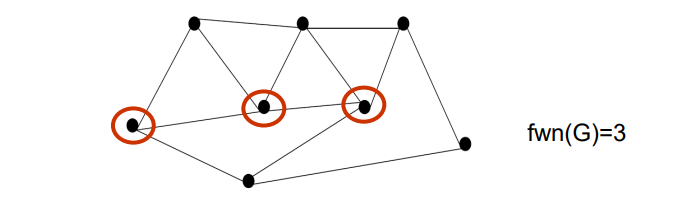
\includegraphics[width=0.7\linewidth]{chapters/images/fixed k.png}
    \caption{Feedback Vertex Number}
    \label{fig:2}
\end{figure}

In questo caso $k$ è fissato.

Ma effettivamente, \textbf{è una buona misura} quella di calcoalre quanti
vertici rimuovere come \textbf{grado di aciclicità}?

\begin{itemize}
    \item Pro: Per $k$ fissato, possiamo controllare in tempo quadratico $fwn(G) = k$
    \item \textbf{Contro}: Grafi semplici possono avere valori FVN grandi
\end{itemize}

\subsubsection{Proposta 2: Feedback Edge Number}
Una misura che ci dice \textbf{quanti archi rimuovere per rendere il grafo
    aciclico}.

A quanto pare, il problema rimane lo stesso.

\begin{figure}[H]
    \centering
    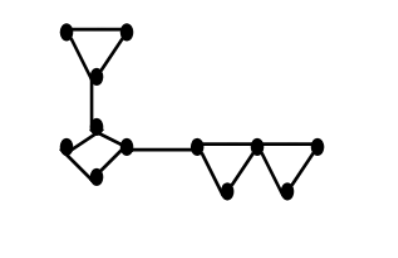
\includegraphics[width=0.7\linewidth]{chapters/images/feg.png}
    \caption{Feedback Edge Number}
    \label{fig:3}
\end{figure}

La soluzione a questi problemi è quella di \textbf{gruppare} i componenti e
creare un cluster.

\subsubsection{Biconnected Width}

\begin{definition}(Biconnected Component)
    Una componente biconnessa è un sottografo massimale che non contiene \textbf{punti di articolazione}, cioè
    un grafo che rimane connesso se rimuovo un nodo del grafo.
\end{definition}

\begin{figure}
    \centering
    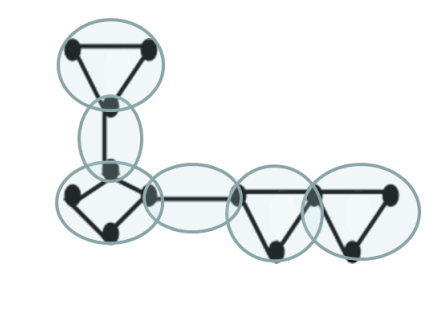
\includegraphics[width=0.7\linewidth]{chapters/images/biconnected.png}
    \caption{Biconnected Component}
    \label{fig:4}
\end{figure}

\begin{itemize}
    \item Pro: bcg(G) può essere calcolato in tempo lineare
    \item \textbf{Contro}: Aggiungere un \textbf{singolo arco} ha un effetto tremendo al bcw(g)
\end{itemize}

\subsubsection{Deep dive nella tree decomposition}

%metti 2 figure sulla stessa riga, g1.png g2.png
\begin{figure}[H]
    \centering
    \begin{minipage}[b]{0.45\linewidth}
        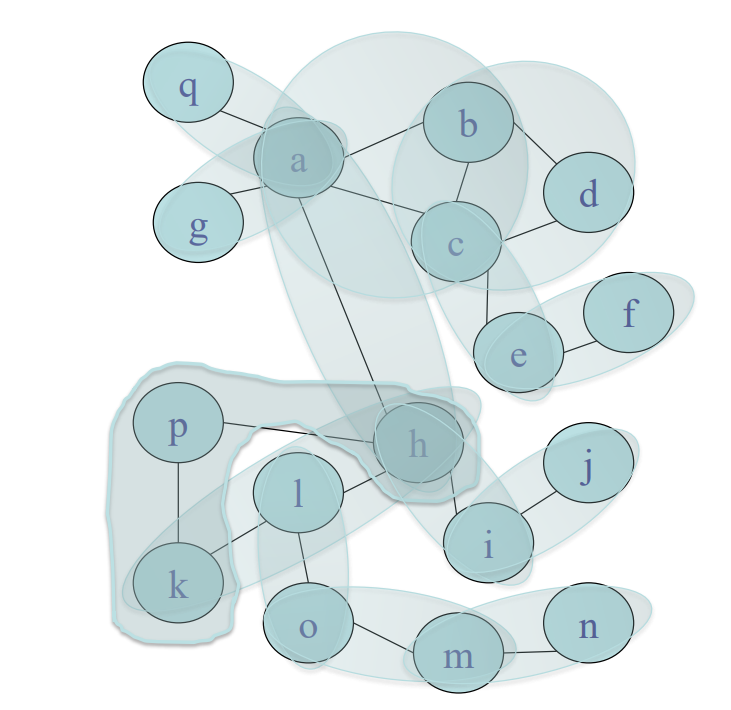
\includegraphics[width=\linewidth]{chapters/images/g1.png}
        \caption{Grafo G1}
        \label{fig:5}
    \end{minipage}
    \hspace{0.5cm}
    \begin{minipage}[b]{0.45\linewidth}
        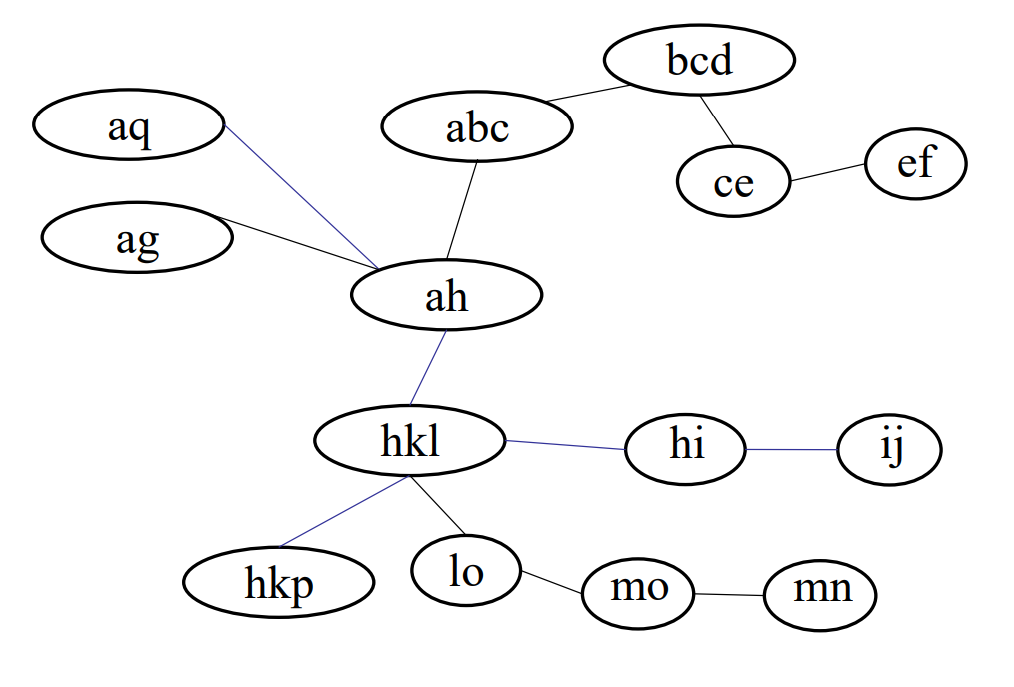
\includegraphics[width=\linewidth]{chapters/images/g2.png}
        \caption{Grafo G2}
        \label{fig:6}
    \end{minipage}
\end{figure}

Entrambe sono la stessa cosa, ma la prima è più \textbf{compatta} della
seconda. La seconda è più \textbf{esplicita}.

\begin{figure}[H]
    \centering
    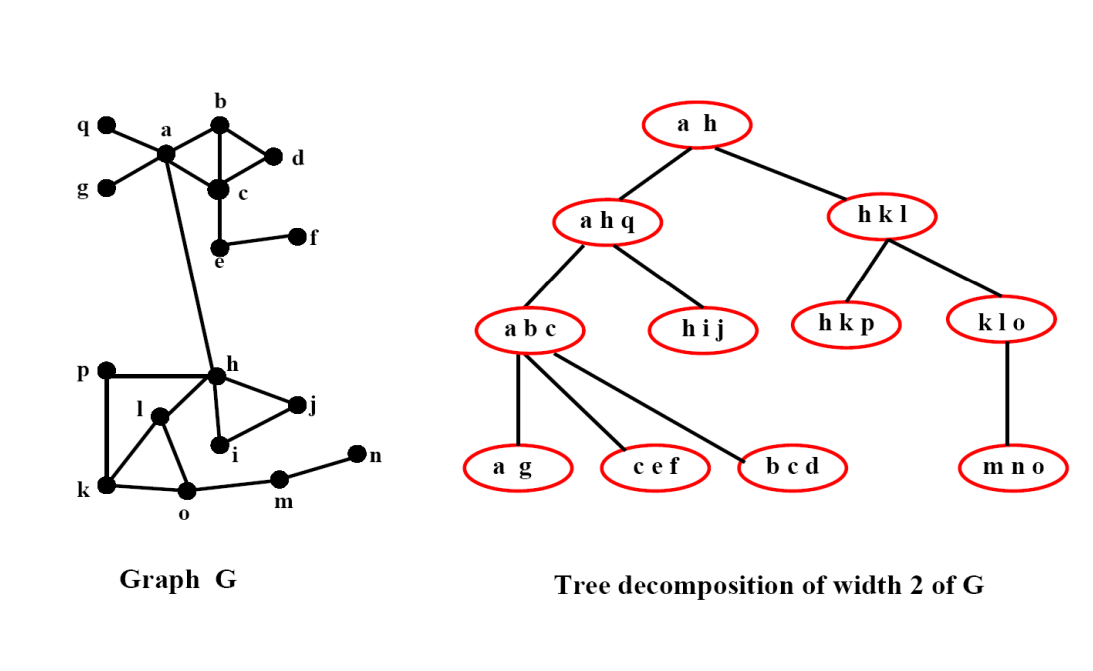
\includegraphics[width=0.7\linewidth]{chapters/images/td.png}
    \caption{Tree Decomposition con width 2}
    \label{fig:7}
\end{figure}

Praticamente, per ogni nodo, si crea un \textbf{bag} che contiene i nodi d
\textbf{vicini} e i nodi \textbf{figli}.

Quali sono le proprietà da rispettare?
\begin{itemize}
    \item Ogni arco deve essere \textbf{coperto}
    \item Se prendo un vertice qualsiasi, il sotto grafo deve rimanere connesso
\end{itemize}
\begin{figure}[H]
    \centering
    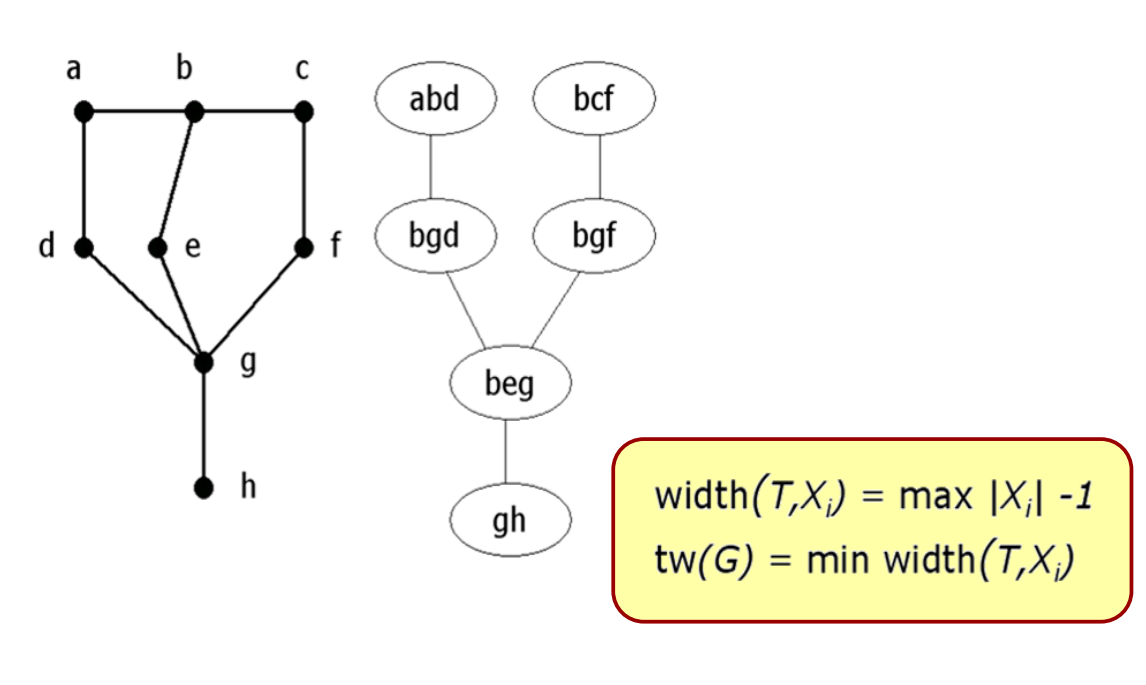
\includegraphics[width=0.7\linewidth]{chapters/images/td2.png}
    \caption{Tree Decomposition con width 2}
    \label{fig:8}
\end{figure}

In questo caso di figura \ref{fig:8} le proprietà sono rispettate!

\textbf{Tree width:} \textit{min width} su tutte le possibili composizioni.
\begin{figure}[H]
    \centering
    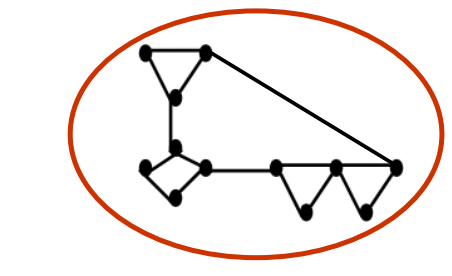
\includegraphics[width=0.7\linewidth]{chapters/images/casostrano.png}
    \caption{Tree Width in caso particolare}
    \label{fig:9}
\end{figure}

In questo caso, cerchiamo di capire come calcolare la \textit{ tree width}.

%abc
%|
%v
%cd
%|
%v
%def
%|
%v
%efg -> fg -> hij -> ikl -> bk

%Fai un grafo con questo

%bk viola la componente biconnessa e devo aggiungerela a tutti i nodi

%abc
%|
%v
%cdb
%|
%v
%defb
%|
%v
%efgb -> fgb -> hijb -> iklb -> bk

%In questo caso, il valore della width è 3

Ma possiamo ottenere un valore migliore? Possiamo ottenere 2?

%abc
%|
%v
%cdb
%|
%v
%dfb
%/   \
%v     v
%dfg   fhb -> hib -> ikb -> bk
%dge           |       | 
% v       v
%hij     ikl

La risposta è \textbf{si}, con questa configurazione posso ottenere una width
di $2$.

Le domande sono 2 ora: \textbf{Come si calcola una decomposizione?} e l'altra è
\textbf{Quando ho una decomposizione, come si risolve un problema NP-Hard?}

\begin{corollary}(Correlazoine NP-Hard e Tree Width)
    Tutti i problemi NP-Hard $2^n \rightarrow 2^k$, cioè avendo $k$ = \textbf{tree width}, i problemi NP-Hard sono risolvibili in tempo $2^k$.
\end{corollary}

\subsubsection{Robber and Cops Game}

\begin{definition}
    Il gioco Robber and Cops è un gioco dove un \textbf{Robber} deve essere catturato da un gruppo di \textbf{Cops}, e
    i Cops possono bloccare le strade per catturare il Robber.

    \begin{itemize}
        \item Input: Un grafo $G$ e un intero $k$
    \end{itemize}
\end{definition}

%2x2 con figure cop1,cop2,cop3,cop4
\begin{figure}[H]
    \centering
    \begin{minipage}[b]{0.45\linewidth}
        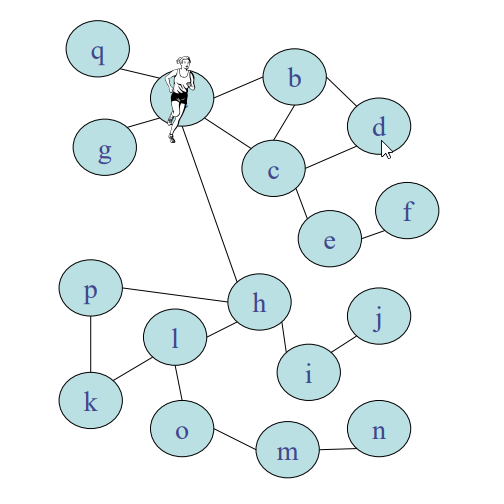
\includegraphics[width=\linewidth]{chapters/images/cop1.png}
        \caption{Cop1}
        \label{fig:5}
    \end{minipage}
    \hspace{0.5cm}
    \begin{minipage}[b]{0.45\linewidth}
        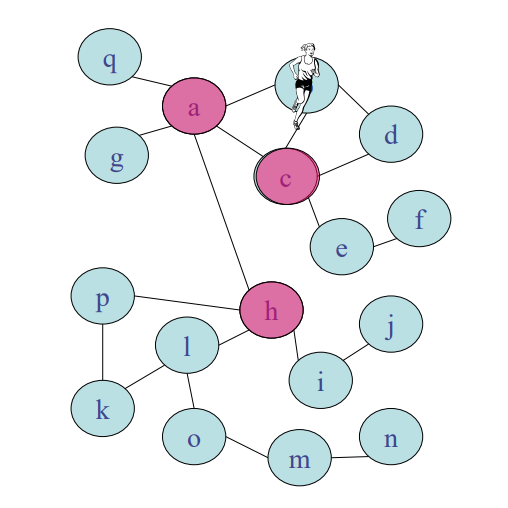
\includegraphics[width=\linewidth]{chapters/images/cop2.png}
        \caption{Cop2}
        \label{fig:6}
    \end{minipage}
\end{figure}

\begin{figure}[H]
    \centering
    \begin{minipage}[b]{0.45\linewidth}
        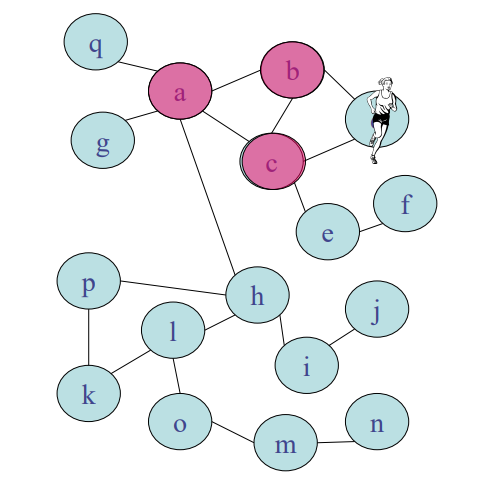
\includegraphics[width=\linewidth]{chapters/images/cop3.png}
        \caption{Cop3}
        \label{fig:5}
    \end{minipage}
    \hspace{0.5cm}
    \begin{minipage}[b]{0.45\linewidth}
        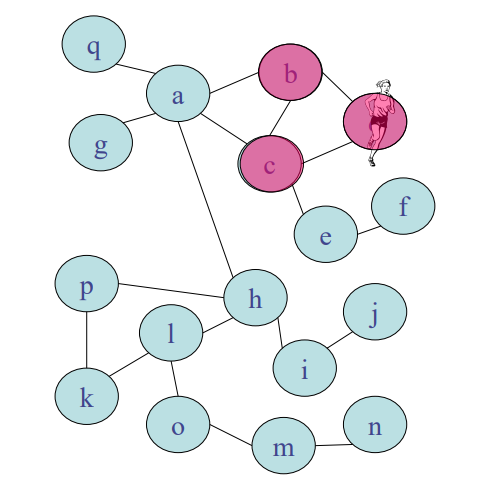
\includegraphics[width=\linewidth]{chapters/images/cop4.png}
        \caption{Cop4}
        \label{fig:6}
    \end{minipage}
\end{figure}

Cosa capiamo da questo? Che cercare di \textbf{vedere le possibili mosse} da
fare per bloccare un ladro nel grafo, praticamente ci tira fuori una
\textbf{struttura} che è una \textbf{tree decomposition.}

\textbf{Nota}: quante combinazioni di stati iniziali ci sono?
\[
    n^k
\]
dove $n$ è il numero di nodi e $k$ è il numero di poliziotti.

\textbf{Nota 2:} Il caso peggiore per una tree decomposition è la \textbf{cricca}.

\begin{definition}(Cricca)
    Una cricca è un sottografo completo, cioè un grafo in cui ogni nodo è collegato a tutti gli altri nodi.
\end{definition}

Un approfondimento algoritmico sulla \textbf{tree decomposition} dovrebbe
essere disponibile alla lezione di \textbf{laboratorio} \ref{MCnets}.

\subsubsection{3 Colorabiltà con Tree Decomposition}

Abbiamo un albero con questi nodi:
\begin{itemize}
    \item yp
    \item yzv
    \begin{itemize}
        \item zvw
        \item vz
    \end{itemize}
\end{itemize}

%fai un albero con questi nodi

Per ogni nodo, prende esattamente $3^k$ per risolvere la 3 colorabilità.

\begin{itemize}
    \item yp:
    \item \begin{itemize}
              \item RB
              \item RG
              \item BG
              \item BR
              \item GR
              \item GB
          \end{itemize}
    \item yzv:
          \begin{itemize}
              \item RBG
              \item RGB
              \item BRG
              \item BGR
              \item GRB
              \item GBR
          \end{itemize}
    \item zvw:
          \begin{itemize}
              \item RBG
              \item RGB
              \item BRG
              \item BGR
              \item GRB
              \item GBR
          \end{itemize}
    \item vz:
          \begin{itemize}
              \item \begin{itemize}
                        \item RB
                        \item RG
                        \item BG
                        \item BR
                        \item GR
                        \item GB
                    \end{itemize}
          \end{itemize}
\end{itemize}

Dove vuole arrivare? Vuole dire che se calcoli le soluzioni per i sotto problemi, si nota che ci sono delle soluzioni che vanno bene anche per alcuni problemi 
più grandi. Quindi si calcolano le \textbf{soluzioni locali} che sono $2^k$ e si utilizzano queste soluzioni per risolvere gli altri. E' quindi praticamente 
un \textbf{algoritmo di programmazione dinamica}.
\newpage
